\input{visualizing_large_text_corpora_praeambel.tex} % Importiere die Einstellungen aus der Präambel
% !TEX root = ./main.tex
% hier beginnt der eigentliche Inhalt
\DeclareUnicodeCharacter{00A0}{ }
\DeclareCaptionLabelFormat{bold}{\textbf{(#2)}}
\captionsetup{subrefformat=bold}

\usetikzlibrary{arrows.meta, babel, decorations.pathreplacing, matrix}
\usepackage{tikz-uml}
\pgfplotsset{width=10cm,compat=1.9}
\addbibresource{bibliographie/bibliographie.bib}

\hypersetup{hidelinks}

% Bagrat Test
%\usepackage[sort&compress]{natbib}


\begin{document}
\pagenumbering{Roman} % große Römische Seitennummerierung
\pagestyle{empty}

% Titelseite //////////////////////////////////////////
\clearscrheadings\clearscrplain

\begin{flushleft}
\begin{normalsize}
Bauhaus-Universität Weimar\\
Fakultät Medien \\
Studiengang Medieninformatik
\vspace{3mm}
\end{normalsize}
\end{flushleft}

\begin{center}
\vspace{20mm}
\begin{LARGE}
Visualisierung der Kategorienstruktur der Wikipedia und Filterung der Ähnlichkeiten von Artikeln auf Basis von Kategorien.\\
\end{LARGE}
\vspace{20mm}
\begin{LARGE}
Bachelorarbeit
\end{LARGE}\\
\vspace{0.4cm}
\vspace{2 cm}

\vspace{1 cm}
\begin{flushleft}Giuliano Castiglia \hfill Matrikelnummer 110656\\
geb. am: 8. Oktober 1991 in Neapel
\end{flushleft}

\vspace{0.5 cm}

\begin{flushleft}
1. Gutachter: Prof. Dr. Bernd Fröhlich\\
2. Gutachter: tba\\
\end{flushleft}

\vspace{1.5cm}
\begin{flushleft}
Datum der Abgabe: 4. September 2017
\end{flushleft}
\end{center}
\clearpage
\pagestyle{useheadings} % normale Kopf- und Fußzeilen für den Rest
\renewcommand*\contentsname{Table of Contents}

% ===============================================================

% Eidesstattliche Erklärung
\addchap{Eidesstattliche Erklärung}

Hiermit versichere ich, dass ich die Bachelorarbeit selbstständig verfasst und keine anderen als die angegebenen Quellen und Hilfsmittel benutzt habe, alle Ausführungen, die anderen Schriften wörtlich oder sinngemäß entnommen wurden, kenntlich gemacht sind und die Arbeit in gleicher oder ähnlicher Fassung noch nicht Bestandteil einer Studien- oder Prüfungsleistung war.

\vspace{3cm}
Weimar, der 2. Oktober 2017

\vspace{1cm}
\noindent\rule{5cm}{0.4pt}\\
GIULIANO CASTIGLIA

\clearpage

% ===============================================================

\addchap{Kurzfassung}
% Destilierte Variante der Thesis
% was ist in der Arbeit entstanden?
% mit Welchen Methoden
% mit welchen Daten

Im Rahmen dieser Arbeit wird eine Visualisierung vorgestellt, welche Kategorien der Wikipedia visuell in Form eines radial angeordneten Baumes darstellt.
Des Weiteren wird ein Verfahren erläutert, welches auf Basis der Wikipedia-Kategorien eine dünn besetzte Matrix von Ähnlichkeiten zwischen Wikipedia-Artikel filtert.
Die Wikipedia dient dabei als Quelle für die Daten.

% Im Rahmen dieser Arbeit wird eine Methode erläutert, welche einerseits die Kategorien der öffentlich zugänglichen Online-Plattform und Enzyklopädie Wikipedia in Form eines radial angeordneten Baumes visuell darstellt, als auch andererseits dazu dienen soll, ein Verfahren zu finden, um eine dünn besetzte Matrix mit Vergleichen zwischen Artikel zu filtern.
Die Informationen über die Kategorien und Artikel werden dabei aus der Wikipedia extrahiert und in einem Format zusammengefasst, welches die visuelle Darstellung der Daten ermöglichen soll.
Dabei wird eine Methode erarbeitet, um aus dem vernetztem Graph von Kategorien, eine hierarchische Baumstruktur zu erhalten.
Diese Baumstruktur soll interaktiv verwendbar sein und eine Exploration der Baumstruktur ermöglichen.
In einem weiterem Teil der Arbeit wird eine Strategie entwickelt, um die dünn besetzte Matrix, von einer Größe von 643\,GB, auf ein Themengebiet einzuschränken und auf diese Weise die sehr umfangreiche Menge an Artikelvergleichen semantisch zu filtern.


\begin{figure}
\centering
\includegraphics[width=\textwidth]{./cover}
% \caption{Die Kategorie \textit{Computer science} bildet als Stammverzeichnis das Zentrum. Alle Kategorien einer Entfernung von drei zur Stammkategorie sind auf konzentrischen Ringen angeordnet.}
% \label{fig:cover}
\end{figure}

% \textit{"However, as we can witness from the example of the Porphyrian tree, the tree of Jesse, the consanguinity tree, Llull's tree of science, and Darwin's tree of life, when sustained by a unique thesis or proposition, a visualization can become an immensely powerful tool and an enduring, contagious meme."}
% \begin{flushleft}
% (Lima 2014, S .43)
% \end{flushleft}

% ===============================================================

\tableofcontents
%\listoffigures
%\listoftables

% ===============================================================

% richtiger Inhalt
\cleardoublepage
\pagenumbering{arabic} % ab jetzt die normale arabische Nummerierung

\chapter{Einleitung}
\label{chap:einleitung}
% !TEX root = ../main.tex
% Einleitung

Das Bedürfnis, Informationen anschaulich darzustellen, ist ein Phänomen, das die Kulturgeschichte des Menschen seit der Frühzeit begleitet. Eine der ältesten visuellen Metaphern ist der Baum.
Dessen grafische Darstellung könnte dabei unterschiedlicher nicht sein, von Abbildungen die nahezu realistisch sind, bis hin zu abstrakten Formen, beispielsweise in Form von einfachen Knoten und Kanten.
Als visuelle Metapher zur Darstellung von Informationen kommen Baumdiagramme in vielen Bereichen zum Einsatz; z.\,B. zur Darstellung von Erbfolgen, der sogenannte Stammbaum, oder um die Rangordnungen im Tierreich abzubilden.
Im Besonderen macht sich diese Darstellungsform folglich die Hierarchie und geordnete Struktur eines Baumes zu Nutzen.
So lässt sich der Baum als eine visuelle Repräsentation verstehen, mit dessen Hilfe sich komplexe Beziehungen zwischen einzelnen Entitäten übersichtlich darstellen lassen.\cite{lima2014book}

Die Arbeit beschäftigt sich einerseits mit der visuellen Metapher des Baums und der darauf aufbauenden Kategorienstruktur von Wikipedia, als auch andererseits mit den Ähnlichkeiten zwischen den einzelnen Paragraphen der in der Wikipedia veröffentlichten Artikeln.
Das Ziel der Arbeit ist es, mittels grafischer Darstellungen und der Möglichkeit der Exploration, das Verständnis über die Datensätze zu verbessern und somit letztlich auch über die Enzyklopädie Wikipedia.

%NOTE
% Relevanz von Informationsvisualisierung\\
% Bezug auf das vorangegangene Projekt Visual Text Analytics\\
% einmal eine Abstrakte Motivation -> Darstellung Kategorienbaum + "Ahnlichkeiten
%
% Motivation aus dem vorg"anger Projekt -> konkreter Bezug auf fehlende Eigenschaften und Erkenntnisse
% defacto die einzige Visualisierung f"ur den Kategoriebaum der Wikipedia
% =========================================================

Die vermeintliche Ordnung der Kategorien innerhalb der Wikipedia von abstrakten und allumfassenden Konzepten auf der höchsten Ebene der Kategorisierung, zu immer spezifischeren Themengebieten, lässt eine stark hierarchische Struktur vermuten.

\section{Motivation}

Im Projekt "`Visual Text Analytics"' wurde bereits ein Versuch unternommen, die Ähnlichkeiten von Wikipedia-Artikeln zu visualisieren.
Der Fokus des Projekts lag auf der Darstellung der inhaltlichen Überschneidungen einer möglichst großen Anzahl von Wikipedia-Artikeln und den Ähnlichkeitswerten zwischen Wikipedia-Artikeln, wie in der Abbildung \ref{fig:vta-cover} gezeigt.
Im Kapitel \ref{subchap:simmatrix}, wird im Detail auf die Berechnung der Ähnlichkeiten eingegangen.
Diese Visualisierung unterstützend werden die zugehörigen Wikipedia-Kategorien in einer separaten Visualisierung als Graph dargestellt.
Dieser die Wikipedia-Katgorien abbildende Graph soll eine verständliche Zusammenfassung auf einer höheren Abstraktionsebene für die Menge der erfassten Wikipedia-Artikel ermöglichen, verdeutlicht in Abbildung \ref{subchap:simmatrix}. 
Dabei werden die Wikipedia-Artikel aus Abbildung \ref{fig:vta-cover}, anhand eines im voraus festgelegten Schwellwerts nach Ähnlichkeiten in Clustern gebündelt.
Die Bestimmung eines initialen Schwellwerts vor der Visualisierung legt dabei fest, bis zu welchem Ähnlichkeitswert Artikel zu Clustern gebündelt werden. Ähnlichkeitswerte unter dem Schwellwert werden nicht mehr in Betracht gezogen. 
Die Änderung des Schwellwerts während der Visualisierung, um Ähnlichkeitswerte in Form von Kanten hinzuzufügen, ist nicht ohne eine Überlappung von Kanten möglich.
Durch die massive Überzeichnen von Elementen ist es nur schwer möglich, aus der Visualisierung etwas zu verstehen. Die damit einhergehende eingeschränkte Interaktivität mit den Daten ist das Grundproblem dieses Projektes.


%Diese Vorgehensweise erschwert jedoch eine dynamische Darstellung, da die Bestimmung eines Schwellwerts die Anordnung der Knoten und Kanten festlegt, weshalb der Schwellwert für die Dauer des Programms statisch bleibt.
%Es besteht die Möglichkeit den Schwellwert zu ändern, doch dadurch würden die neu gezeichneten Kanten so angeordnet, dass eine Vielzahl an Überlappungen entstünden.

% \paragraph{Ziel}
Den Impuls zur vorliegenden Arbeit gaben die Beobachtungen aus diesem Projekt \emph{Visual Text Analytics}.
Im Laufe der Projektarbeit wurden Schwachstellen identifiziert und Mängel herausgestellt, die im Rahmen dieser Untersuchung weiterbearbeitet wurden.
Der Fokus dieser Forschungsarbeit liegt dabei auf der Entwicklung einer geeigneten Darstellung von Verbindungen zwischen den Kategorien der Wikipedia.
Eine Anforderung, die an eine Visualisierung von Informationen gestellt wird, ist, Knoten und Kanten zu finden, bei denen die Überlappung möglichst gering ist. Zugleich soll auch eine mögliche Anpassung des Schwellwerts gewährleistet werden, dass die Überlappungen der dargestellten Elemente weiterhin möglichst niedrig bleibt.
Die Suche nach den Kategorien und die interaktive Exploration der Verbindungen zwischen den Kategorien steht dabei im Mittelpunkt.
Des Weiteren setzt sich die Arbeit mit der Entwicklung einer Strategie auseinander, um eine dünn besetzte Matrix in der Größe von 643 GB zu veranschaulichen und zugänglich zu machen.
Die Arbeit zielt darauf ab, das Verständnis über die Enzyklopädie Wikipedia zu schärfen und zu vertiefen.


\begin{figure}
\centering
\includegraphics[width=\textwidth]{images/01_introduction/vta-cover.png}
\caption{Ausschnitt aus dem Projekt \textit{Visual Text Analtytics}. Rechts unten ist ein Cluster im Fokus zu sehen. Der Hintergrund zeigt die Startvisualisierung mit einer Übersicht aller Cluster.}
\label{fig:vta-cover}
\end{figure}

\begin{figure}
    \centering
    \includegraphics[width=\textwidth]{images/01_introduction/category-view.png}
    \caption{Ausschnitt des Kategoriengraphen. Die Knoten stellen Kategorien dar und die Kanten veranschaulichen die Verbindungen zwischen den Kategorien.\\ In diesem Bild wird die grün gefärbte Kategorie ausgewählt. Alle Knoten und Kanten ohne Verbindung zur ausgewählten Kategorie sind ausgegraut.}
    \label{fig:category-view}
\end{figure}
\todotext{bild mit einer geclickten Kategorie}










% DRAFTS ============================
% Um die enorme Menge an Kanten, welche einen Vergleich zwischen zwei Artikeln repres"antiert, darstellen zu k"onnen, muss ein Schwellwert festgelegt werden, bevor die Visualisierng ausgef"uhrt wird.

% Ziel der Arbeit ist es, das Verst"andnis "uber die Kategoriestruktur und die "Ahnlichkeiten zwischen Artikeln der Wikipedia zu verbessern.
% F"ur die enorme Menge an Vergleichen zwischen Artikeln muss eine L"osung entwickelt werden, welche die Menge reduziert, somit f"ur den Computer darstellbar und f"ur den Menschen nachvollziehbar ist.
% Der Mittelpunkt der Arbeit ist die Darstellung der hierarchischen Struktur der Kategorien aus der Wikipedia.

% BULLET LIST ++++++++++++++++++++++++++++++++++++++++++++++++
% \begin{itemize}
%   \item Bedeutung des Wikipediadatensatzes
%   \item Kritikpunkte im Projekt Visual Text Analytics
%   \begin{itemize}
%     \item statisches Layout
%     \item fehlende M"oglichkeit zur Exploration der Daten
%     \item "Ubersicht der Visualisierung ist sehr undurchsichtig
%     \item Schwierigkeiten beim Nachvollziehen der Verbindungen zwischen den Artikeln untereinander
%     \item "Anderung des Schwellwertes f"ur "Ahnlichkeiten -> zu viele Kanten
%     \item fehlende M"oglichkeit, die Auswahl an Artikeln einzuschr"anken
%     \item Unterst"utzende Funktion zum Zusammenfassen von mehreren Artikeln -> Kategorien, Cluster
%     \item Artikelcluster mit vielen "Ahnlichkeiten zueinander sind schwer zu lesen
%     \item Kategorienbaum unzureichend als Unterzt"utzung neben den Artikeln
%   \end{itemize}
% \end{itemize}


% \begin{itemize}
%     \item Verbesserung des Verst"andnisses des "Ahnlichkeitsma"ses
%     \item Darstellung der Hierarchie von Kategorien
%     \begin{itemize}
%       \item Konstruktion eines Kategorienbaumes mit der M"oglichkeit der Exploration
%     \end{itemize}
%     \item Interaktive Visualisierung
%     \begin{itemize}
%       \item "Anderung des Schwellwerts zur Laufzeit
%     \end{itemize}
%     \item Exploration der Daten
%     \item Bezug zu anderen Datens"atzen: Autoren, Editierungen, etc.
% \end{itemize}














































% % ////////////////////////////////////
% \begin{figure}[H]
%     \centering
%     \begin{subfigure}[b]{0.96\textwidth}
%         \includegraphics[width=\textwidth]{images/01_introduction/motivation_temporal_superresolution_one.pdf}
%         \caption{3D video playback rate matching the low recording rate}
%         % \label{subfig:playback_rate_matching}
%     \end{subfigure}

% 	\vspace{1.0cm}

%     \begin{subfigure}[b]{0.96\textwidth}
%         \includegraphics[width=\textwidth]{images/01_introduction/motivation_temporal_superresolution_two.pdf}
%         \caption{3D video playback matching the video encoding standards to ensure persistence of fluid motion}
%         % \label{subfig:playback_rate_higher}
%     \end{subfigure}
%     \caption[Concept of Temporal Super Resolution in a 3D Video Player]{In this Figure, two different playback rates for a low frame rate recording of a 3D volume sequence is presented. The tick marks on the black arrows indicate the position of recorded frames. The blue arrows indicate the playback rate that matches the recording \subref{subfig:playback_rate_matching} and an increased playback rate \subref{subfig:playback_rate_higher} using temporal interpolation to provide the viewer with a impression of fluid motion. }
%     % \label{fig:temporal_superresolution}
% \end{figure}

%  \cite{VillanuevaEtAl:2016}

\chapter{Related Work}
\label{chap:related_work}
% !TEX root = ../main.tex

Im Forschungsfeld der Informationsvisualisierung ist die Wikipedia eine häufig verwendete Datenquelle und stellt aufgrund ihres komplexen Aufbaus und ihrer enormen Größe eine besondere Herausforderung in diesem Bereich dar.\\
In der Arbeit von Holloway~\cite{holloway2007analyzing} wird die inhaltliche Reichweite der Wikipedia in Form einer \emph{Category Map} dargestellt.
Dafür werden genau diejenigen Kategorien durch eine Kante miteinander verbunden, die mindestens einen gemeinsamen Artikel haben. Auf Basis dieser neuen Verbindungen wird ein Kategoriengraph gezeichnet.
\begin{figure}[H]
    \centering
    \includegraphics[scale=.14]{images/hol-wikivis3}
    \caption{Karte von Kategorien angeordnet nach der Methodik von Holloway~\cite{holloway2007analyzing}.}
    \label{fig:hol-wikivis}
\end{figure}
Darüber hinaus wird ein Gewicht eingeführt, das die Stärke dieser Verbindungen abbilden soll.
Das Gewicht ist eine Modifikation der Kosinusähnlichkeit.
Um die inhaltliche Reichweite des dargestellten Graphen deutlicher hervorzuheben, werden die \emph{Main Topic Categories} beschriftet und die Kategorien farblich markiert, die in ihrem Titel besonders häufige auftretende Wörter enthalten.
Die Abbildung~\ref{fig:hol-wikivis} zeigt diese \emph{Category Map}.\\
Die Arbeit \emph{Wikiviz: Visualizing Wikipedia}~\cite{harrison2006wikiviz} stellt den Graphen von Verbindungen zwischen Kategorien dar, um ungewöhnliche Verbindungen zwischen Kategorien zu veranschaulichen, wie in der Abbildung~\ref{fig:harr-wikiviz} zu erkennen.
Ausgehend von einer Startkategorie werden die Verbindungen bis zur Tiefe 5 gezeichnet.
Darüber hinaus liegen die Kategorien, die untereinander viele Verbindungen besitzen, näher beieinander als solche, die weniger Verbindungen untereinander aufweisen.

Für die Anordnung der Kategorien entwickelt Harrison in seiner Arbeit eine eigene Methode, da die Ansätze wie \emph{Force-Directed-Layout} nach~\cite{fruchterman1991graph} und~\cite{kamada1989algorithm} zu rechenintensiv sind und sich deshalb die Laufzeit der Algorithmen mit einer steigenden Anzahl an Kategorien verlängert.
Die Informationen über die Verbindungen von Kategorien werden direkt aus den Wikipedia-Seiten extrahiert, da die Daten aus der Wikipedia-Datenbank zu unpräzise sind~\cite{harrison2006wikiviz}.
\begin{figure}[H]
    \centering
    \includegraphics[width=\textwidth]{images/har-wikiviz}
    \caption{WikiViz \cite{harrison2006wikiviz}}
    \label{fig:harr-wikiviz}
\end{figure}
Auf ähnliche Weise wie Holloway behandelt die Arbeit von Biuk-Aghai~\cite{biuk2011wikipedia} die inhaltliche Reichweite der Wikipedia.
Die Anordnung der Daten erfolgt bei Biuk-Aghai entsprechend dem \emph{Radial Convergence Model} nach Lima~\cite[S.~63]{lima2017circle}.
Die Visualisierung übersetzt die Größe der \emph{Top-Level}-Kategorien anhand der Anzahl der enthaltenen Artikel in einen Balken auf dem äußeren Ring. Vertiefend werden die direkten Unterkategorien mit ihren Titeln weiter außen im Ring gezeichnet, um die \emph{Top-Level} Kategorien detailreicher zu umschreiben.
Innerhalb des Rings werden alle Artikel als Knoten dargestellt, wobei die Position eines Knotens von der Ähnlichkeit des zugehörigen Artikels zu den Kategorien abhängig ist.
% Die Arbeit von Picandet \cite{picandet2014wikiabout} versucht auf die selbe art die 


In der Arbeit \emph{ClusterBall} von Harrison~\cite{harrison2006clusterbal} werden Wikipedia-Kategorien in einem \emph{Radial Convergence Model}~ \cite[S.~63]{lima2017circle} angeordnet.
Im Fokus der Visualisierung steht die Bildung und Darstellung von \emph{Kategorienclustern}.
Infolgedessen werden die Kategorien in drei unterschiedliche Gruppen eingeteilt: Erstens eine Startkategorie im Zentrum der Darstellung, zweitens Kategorien auf dem äußeren Ring und drittens solche Kategorien, die sich innerhalb des Ringes befinden.
Die Kanten bilden die Verbindungen zwischen den Kategorien ab und sind, je nach ihrer Gruppenzugehörigkeit, unterschiedlich gefärbt.
Die Kategorien auf dem äußeren Ring werden so angeordnet, dass die Kantenlänge minimiert wird, was wiederum zu einer eindeutig erkennbaren Bildung von \emph{Clustern} führt.
Die Kategorien innerhalb des Rings, in der Abbildung~\ref{fig:harr-cluster} als blaue Knoten zu erkennen, bilden ein \emph{Cluster}. 

\begin{figure}[H]
    \centering
    \includegraphics[width=\textwidth]{images/clusterball}
    \caption{Clusterball \cite{harrison2006clusterbal}}
    \label{fig:harr-cluster}
\end{figure}

Die Visualisierung von Clever~\cite[S.~233]{lima2017circle} stellt die Hierarchie des Kategoriensystems der Nationalbibliothek der Niederlande dar.
Auch Clever verwendet eine radial angeordnete hierarchische Struktur.
Seine Visualisierung unterscheidet jedoch farblich nicht zwischen Kategorien der ersten Ebene und Kategorien niedrigerer Ebenen.
Die Herangehensweise von Clever, die Kategorienhierarchie zur Ordnung und Suche in Archiven zu nutzen, liefert einen Impuls für die vorliegende Arbeit.



% \section{Graphen und B"aume}
% MoireGraphs: Radial Focus+Context Visualization and Interaction for Graphs with Visual Nodes \cite{jankun2003moiregraphs}
% RINGS : A Technique for Visualizing Large Hierarchies \cite{teoh2002rings}
% Visualization of Large Hierarchical Data by Circle Packing \cite{wang2006circlepacking}

% \section{Radiales Layout}

% A parent-centered radial layout algorithm for interactive graph visualization \cite{pavlo2006parent}







\chapter{Daten}
\label{chap:daten}
% Daten

\section{"Ahnlichkeitsmatrix}
\begin{itemize}
    \item Bezugnahme zur Thesis von Tristan Licht
    \item Inhalt der Matrix
\end{itemize}

\section{Wikipedia XML Dump}
\begin{itemize}
    \item Datenstruktur des Wikipediakorpus
    \item Notwendige Metainformationen aus dem Korpus
\end{itemize}



\section{Datenbankentwurf}
\begin{itemize}
    \item Erl"auterung der Datenbankstruktur
\end{itemize}


\section{Ablauf der Datenverabeitung}
\begin{itemize}
    \item Aufbereitung der Rohdaten: S"auberung, Formatierung
    \item Erstellung der Datenbank
\end{itemize}


\chapter{Visualisierung}
\label{chap:visualization}
% !TEX root = ../main.tex
% Visualisierung

% Kapitel \ref{chap:daten} gibt einen "Uberblick "uber gr"o"se und Struktur der genutzten Datens"atze um nachvollziehen zu k"onnen welche Daten visualisiert werden.
In diesem Kapitel wird auf die gewählte Darstellung von Kategorien eingegangen und welche Interaktionsmöglichkeiten die Visualisierung bietet.
Darüber hinaus wird verdeutlicht, welche nicht sichtbaren Veränderungen während der Laufzeit des Programms an den Daten vorgenommen werden.
In diesem Kapitel werden die beschriebenen Datensätze aus dem Kapitel \ref{chap:daten} näher erläutert und mit ihrer visuellen Repräsentation verknüpft.

Im Gegensatz zur Visualisierung aus dem Projekt \emph{Visual Text Analytics} stehen die Verbindungen zwischen den Kategorien im Mittelpunkt der angestrebten Darstellung.
Der Ansatz aus dem vorangegangenen Projekt, möglichst viele Artikel mit ihren Ähnlichkeiten abzubilden, führt zu einer unüberschaubaren Menge an Vergleichen, die wiederum in einer Undurchsichtigkeit der dargestellten Elemente resultiert (\emph{visual clutter}).
In der vorliegenden Arbeit wird deshalb ein neuer Ansatz verfolgt, welcher sich auf die Kategorien fokussiert.
Mittels der Kategorien soll ein abstrakterer Zugang zu den Artikeln geschaffen, die Übersichtlichkeit gestärkt und die Auswahl an Artikeln auf ein Themengebiet beschränkt werden.

%  Vorhaben, eine geeignete Darstellungsform der Kategorienstruktur zu finden, folgend wird diese Struktur analysiert.
% % Die Voraussetzung dafür ist die Analyse der Kategorienstruktur der Wikipedia 
Der Grundgedanke der Arbeit liegt in der Annahme, die Kategorienstruktur als eine Hierarchie von Abstraktionsebenen zu interpretieren.
Diese Annahme wird durch eine Analyse der Kategorienstruktur überprüft.
Auf der Wikipedia-Seite \emph{Main Topic Classifications}\footnote{\url{https://en.wikipedia.org/wiki/Category:Main_topic_classifications}} wird darauf hingewiesen, dass die Kategorienstruktur nicht als strikt hierarchisch zu verstehen ist.
Daraus lässt sich schließen, dass die Kategorien in einem Graphen miteinander verbunden sein können.
Die genauere Betrachtung der Beziehungen zwischen den Kategorien verdeutlicht ihre Eigenschaften.
Besteht eine Verbindung zwischen zwei Kategorien, werden diese jeweils in der anderen Kategorie als Unterkategorie oder als Oberkategorie eingetragen. 
Daraus lässt sich folgern, dass der Graph, bestehend aus Verbindungen zwischen den Kategorien, ein gerichteter Graph ist und somit einer gewissen Ordnung folgt.

Im Folgenden wird an einem konkreten Beispiel ein Pfad von Unterkategorien exemplarisch erkundet.
Die Analyse der Wikipedia-Seite der Kategorie \emph{Computer science} und ihrer Unterkategorien zeigt, dass die Kategorien, die näher zum gewählten Stammverzeichnis \emph{Computer science} liegen, Themengebiete eher umfassend beschreiben.
Die Kategorien, die weiter vom Stammverzeichnis entfernt sind, umschreiben einen Gegenstand hingegen spezifischer.
Auf Grund dieser Beobachtungen kann davon ausgegangen werden, dass die Kategorienstruktur einer thematischen Ordnung bzw. einer thematischen Hierarchie folgt.
Am Beispiel eines Pfades der Unterkategorien des Stammverzeichnisses \emph{Computer Science} werden diese Abstraktionsebenen exemplarisch in der Abbildung~\ref{fig:cs-tree} dargestellt.

\begin{figure}
    \centering
    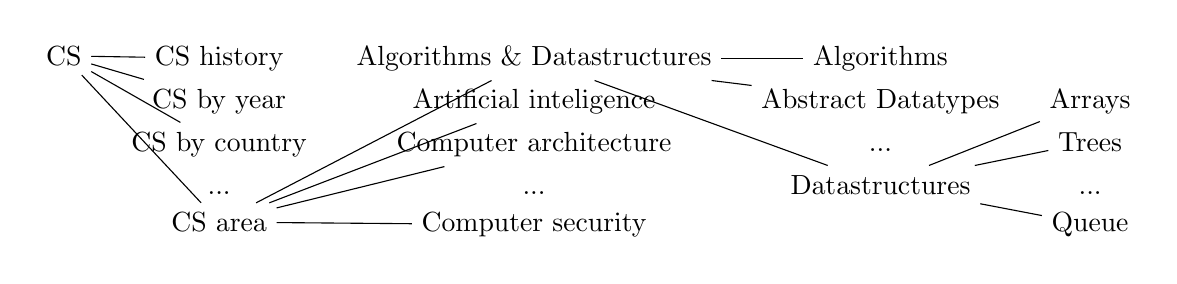
\begin{tikzpicture}
    \matrix (m) [matrix of nodes, column sep=4mm]
    {
        CS  & CS history                & Algorithms \& Datastructures          & Algorithms            &   \\
            & CS by year                & Artificial inteligence               &  Abstract Datatypes   & Arrays  \\
            & CS by country             & Computer architecture                 &  ...                  & Trees  \\
            & ...                       & ...                                   & Datastructures        & ...  \\
            & CS area                   & Computer security                     &                       & Queue  \\
    };
    \draw (m-1-1) -- (m-1-2);
    \draw (m-1-1) -- (m-2-2);
    \draw (m-1-1) -- (m-3-2);
    \draw (m-1-1) -- (m-5-2);
    
    \draw (m-5-2) -- (m-1-3);
    \draw (m-5-2) -- (m-2-3);
    \draw (m-5-2) -- (m-3-3);
    \draw (m-5-2) -- (m-5-3);
    
    \draw (m-1-3) -- (m-1-4);
    \draw (m-1-3) -- (m-2-4);
    \draw (m-1-3) -- (m-4-4);
    
    \draw (m-4-4) -- (m-2-5);
    \draw (m-4-4) -- (m-3-5);
    \draw (m-4-4) -- (m-5-5);
    

    \end{tikzpicture}
    \caption{Ausschnitt der Kategorienstruktur ausgehend von der Kategorienseite \emph{Computer science}}
    \label{fig:cs-tree}
\end{figure}

Zusammenfassend lässt sich aus den vorangegangenen Beobachtungen Folgendes schließen: Die Kategorien folgen untereinander einer Ordnung, welche durch die gerichteten Verbindungen zwischen den Kategorien abgebildet werden.
Diese Feststellung bildet die Basis, um aus dem gerichteten Graphen einen Baum zu konstruieren, der die Hierarchie der Kategorien abbildet.\\
Weiterhin besteht die Schwierigkeit darin, die Entstehung der Schleifen im Kategorienbaum zu verhindern und somit zu entscheiden, welche Kanten aus dem gerichteten Kategoriengraphen in den Kategorienbaum übernommen werden.
Die Konstruktion eines Baumes, der die Hierarchie abbilden soll, stellt somit kein triviales Problem dar.

Die in dieser Arbeit angewandte Methode traversiert den gerichteten Kategoriengraphen mit einer iterativen Tiefensuche, auf die im Kapitel \ref{chap:Implementierung} näher eingegangen wird, ausgehend von einer gewählten Startkategorie.
Dabei werden nur die Knoten aus dem Graphen dem Baumdiagramm hinzugefügt, die nicht bereits in diesem abgebildet sind.
Die Knoten einer Ebene werden mit dem Knoten verbunden, von dem aus eine Kante auf sie gerichtet ist.
Auf diese Art soll gewährleistet werden, dass keine Schleifen während der Konstruktion des Baumes entstehen.
In dem Kapitel~\nameref{chap:Implementierung} wird auf den verwendeten Algorithmus, welcher aus dem gerichteten Graphen ein Baumdiagramm konstruiert, näher eingegangen.

Der erste Ansatz versucht einen Kategorienbaum für \emph{sämtliche} Wikipedia-Kategorien zu erstellen.
Für einen vollständigen Kategorienbaum wird ein Stammverzeichnis gesucht, das zwei Eigenschaften erfüllt: Erstens sollen in den Unterkategorien, ausgehend vom Stammverzeichnis, ausschließlich Kategorienseiten oder Artikelseiten eingetragen sein und zweitens soll ein Stammverzeichnis so gewählt werden, dass möglichst viele Themengebiete direkt oder in Unterkategorien enthalten sind.
Die Wikipedia markiert die Kategorie \emph{Contents}\footnote{\url{https://en.wikipedia.org/wiki/Category:Contents}} als Stammverzeichnis aller Kategorienseiten.
Diese Seite ist gleichwohl ungeeignet für die Nutzung als Stammverzeichnis, da in ihr auch Kategorien aus Namensräumen außerhalb der Artikelseiten eingetragen sind.

In dieser Arbeit wird die Kategorie \emph{Main Topic Classifications} als globales Stammverzeichnis für alle Kategorien gewählt, da sie all diese Eigenschaften erfüllt.
In ihren Unterkategorien sind hauptsächlich Artikelseiten eingetragen. 
Die direkten Unterkategorien enthalten 22 unterschiedliche Themengebiete, die den Inhalt der Wikipedia abbilden.

Sucht ein Nutzer nach einer Kategorie, ist es folglich möglich, ihm, ausgehend von der gesuchten Kategorie, einen Ausschnitt des vollständigen Kategorienbaums zu zeigen.
Das Problem der dargestellten Hierarchie ist, dass bestimmte Verbindungen der gesuchten Kategorie oder ihren Unterkategorien nicht dargestellt werden, weil sie bereits in einem höheren Pfad des vollständigen Kategorienbaums abgebildet sind.
In der Abbildung~\ref{fig:two-trees} wird dieses Phänomen verdeutlicht.

\begin{figure}
    \centering
    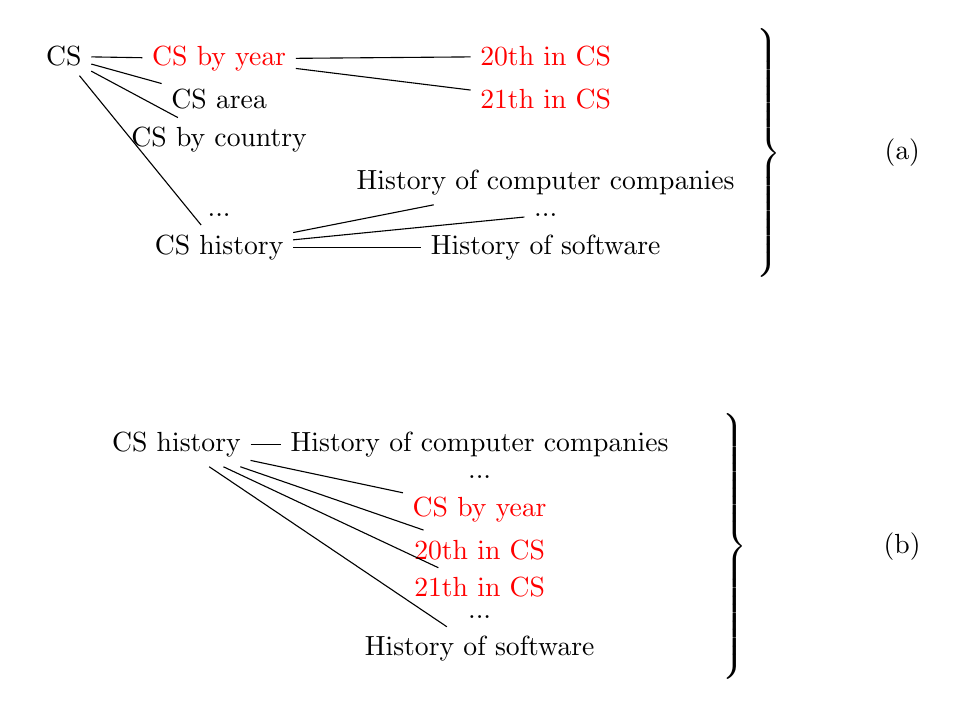
\begin{tikzpicture}
        \matrix (m) [matrix of nodes, column sep=4mm, right delimiter=\}] at (0,5)
            {
                CS  &|[red]|CS by year        &|[red]| 20th in CS                    \\
                    & CS area           &|[red]| 21th in CS                    \\
                    & CS by country     & \\
                    &                   & \\
                    &                   & History of computer companies \\
                    & ...               & ...                           \\
                    & CS history        & History of software           \\
            };
            \draw (m-1-1) -- (m-1-2);
            \draw (m-1-1) -- (m-2-2);
            \draw (m-1-1) -- (m-3-2);
            \draw (m-1-1) -- (m-7-2);
            
            \draw (m-1-2) -- (m-1-3);
            \draw (m-1-2) -- (m-2-3);
            \draw (m-7-2) -- (m-5-3);
            \draw (m-7-2) -- (m-6-3);
            \draw (m-7-2) -- (m-7-3);
            
            % \draw[thick, blue ] (-4,5) rectangle (5.2,3);
            \node (a) at (6.5,5) {(a)};
            \node (b) at (6.5,0) {(b)};

        \matrix (l) [matrix of nodes, column sep=4mm, right delimiter=\}] at (0,0)
            {
                & CS history  & History of computer companies                    \\
                &             & ...                 &        \\
                &             & |[red]|CS by year          & \\
                &             & |[red]|20th in CS          & \\
                &             & |[red]|21th in CS          &  \\
                &             & ...                 &   \\
                &             & History of software &          \\
            };
            \draw (l-1-2) -- (l-1-3);
            \draw (l-1-2) -- (l-3-3);
            \draw (l-1-2) -- (l-4-3);
            \draw (l-1-2) -- (l-5-3);
            \draw (l-1-2) -- (l-7-3);



    \end{tikzpicture}
    \caption{Es werden zwei Kategorienbäume dargestellt, die mit den unterschiedlichen Anstäzen aus \ref{chap:visualization} konstruiert wurde. Rot markierte Kategorien aus Abbildung (b) sind in Abbildung (a) nicht unter der Kategorie \emph{CS History eingetragen}, stattdessen sind die markierten Kategotrien in anderen Pfanden des Kategorienbaums}
    \label{fig:two-trees}
\end{figure}

Der zweite Ansatz probiert, diese Ungenauigkeit in der Darstellung der Hierarchie aus dem gerichteten Graphen zu mindern.
Sucht der Nutzer nach einer Kategorie, wird, wie bereits am Anfang des Kapitels beschrieben, mit der iterativen Tiefensuche und den festgelegten Bedingungen ein neuer Kategorienbaum konstruiert.
% Dieser unterscheidet sich vom Ausschnitt des vollständigen Kategorienbaums aus dem ersten Ansatz, wie in der Abbildung~\ref{fig:two-trees} veranschaulicht wird.
Da in diesem Fall der Kategoriengraph ausgehend von der gewählten Wurzelkategorie traversiert wird, werden mehr Unterkategorien in der Hierarchie abgebildet als zuvor in dem Ansatz des vollständigen Kategorienbaums.
Dieser Kategorienbaum schafft ein genaueres Abbild der Hierarchie für die gewählte Wurzelkategorie.
Dabei ist zu beachten, dass die dargestellte Hierarchie immer nur eine Interpretation des gerichteten Graphen bedeutet.

In beiden Fällen wird jedoch mit der Hierarchie der Kategorien eine \emph{Top-Down}-Struktur\footnote{\url{https://de.wikipedia.org/wiki/Top-down_und_Bottom-up}} modelliert, die genutzt werden kann, um Themengebiete zu erkunden.
Der Abschnitt~\ref{subchap: filter-vis} erklärt, wie die \emph{Top-Down}-Exploration genutzt wird, um auf Artikel zuzugreifen.
Dieser Ansatz spielt eine grundlegende Rolle in der Selektion der Artikel.
In den folgenden Abschnitten wird auf die visuelle Umsetzung und die Interaktion eingegangen.

\begin{figure}[H]
    \centering
    \begin{tikzpicture}
    \node[draw=red, very thick] (fig) at (3,3) {\includegraphics[width=\textwidth]{images/start-half}};
    \node[red, below] at (fig.south) {(a)};
    
    \node (one) at(-2.6,7.7) [rectangle, draw=red, very thick, inner sep=0pt, minimum width=5.2cm, minimum height=1.5cm]{};
    \node[red, below] at (one.south) {(b)};
    
    \node (two) at(7.85,7.9) [rectangle, draw=red, very thick, inner sep=0pt, minimum width=6.6cm, minimum height=.77cm]{};
    \node[red, above] at (4.5, 6.6){(c)};
    \node (three) at(8.75,7.1) [rectangle, draw=red, very thick, inner sep=0pt, minimum width=4.8cm, minimum height=.6cm]{};
    \node[red, below] at (three.south) {(d)};
    \end{tikzpicture}
    \caption{In der Darstellung der Kategorie \emph{Computer science} sind die Unterkategorien im Zentrum des radialen Graphen mit einer Tiefe von 1 mit der Stammkategorie verbunden und sichtbar.\\ (a) Hauptfenster, (b) zusammenfassende Statistik über vorhandene Daten, (c) Suchleiste, (d) Regler zur Änderung des Schwellwerts}
    \label{fig:small-start}
\end{figure}


\section{Layout} \label{subchap:layout}

In dieser Arbeit werden Ausschnitte der Kategorienstruktur der Wikipedia, welche sich insgesamt auf etwa $1.4$~Millionen Seiten beläuft, siehe die Tabelle \ref{tab:xml-overview}, dargestellt.
Wie einleitend in diesem Kapitel beschrieben, werden die Kategorien der Wikipedia in Form eines hierarchischen Baums modelliert.
Die Veränderung der Baumdarstellung durch das Hinzufügen von Knoten wird ebenfalls ermöglicht. 
Es gibt verschiedene Varianten, Bäume anzuordnen. 
Bekannte Methoden sind die horizontale und die vertikale Ausrichtung von Baumdarstellungen.
Die enorme Menge an möglichen Kategorien, die dargestellt werden sollen, erfordert eine Methode, welche den vorhandenen Platz des Computer-Bildschirms voll ausschöpft und dabei die Anordnung von Knoten in kurzer Zeit, also möglichst ohne Verzögerung, berechnet.
Hierfür werden wiederum zwei Ansätze getestet, welche nachfolgend erläutert werden.\\
Der erste Versuch wird mit dem Algorithmus nach Fruchtermann et al. \cite{fruchterman1991graph} implementiert.
Diese Arbeit verwendet eine Implementierung des Algorithmus aus der \emph{Boost Graph Library} \footnote{\url{http://www.boost.org/doc/libs/1_65_1/libs/graph/doc/index.html}}. Die Standardeinstellungen der Parameter dieses Algorithmus werden beibehalten.
In diesem Versuch stellt sich heraus, dass die Berechnung der Knoten anhand eines physikalischen Modells ab einer gewissen Größe zu rechen- und zeitintensiv wird, sodass keine Interaktion mit der Darstellung möglich ist.
Ein weiteres Problem dieses Ansatzes ist die Positionierung der Knoten.
Aus der Anordnung der Knoten nach dem Algorithmus von Fruchtermann et al.~\cite{fruchterman1991graph} lässt sich die hierarchische Struktur der Kategorien nur schwer erkennen. 
Folglich ist der Algorithmus in dieser Form nicht optimal für die Darstellung des Kategorienbaums und wird deshalb in dieser Arbeit nicht weiter verfolgt.

Der zweite Ansatz versucht die Anordnung der Knoten des Kategorienbaums mit dem Algorithmus nach Eades \cite{eades1991drawing} zu realisieren.
Die Positionierung der Knoten erfolgt in einem polaren Koordinatensystem, dabei stellt die Wurzelkategorie den Ursprung dieses Systems dar.
Die Distanz und der Winkel zum Ursprung geben die Position eines Knotens an.
Der Algorithmus ermöglicht es, dass jegliche Knoten einer Baumdatenstruktur als Wurzel für die Darstellung gewählt werden können. Anhand des ausgesuchten Knotens werden alle anderen Knoten in konzentrischen Ringen um den Wurzelknoten angeordnet.
Die Größe eines Sektors innerhalb des polaren Koordinatensystems, welcher für einen Teilbaum belegt wird, ist davon abhängig, wie viele Knoten sich in dem Teilbaum befinden.
Ausschlaggebend für die Größe des Sektors ist dabei die Anzahl an Blattknoten des jeweiligen Teilbaums, siehe hierzu Eades \cite[S.~15]{eades1991drawing}.
Der Algorithmus garantiert, dass die Anordnung des Baumes planar ist, also keine Überlappungen entstehen. \cite[S.~16]{eades1991drawing}.
Der Algorithmus erfüllt zudem die oben beschriebenen Voraussetzungen zur Darstellung des Kategorienbaumes.

\begin{figure}[H]
    \centering
    \includegraphics[width=\textwidth]{images/cat-size-direct}
    \caption{Die Anzahl der Artikel einer Kategorie wird direkt auf die Größe des Knotens der Kategorie übertragen}
    \label{fig:cat-size-direct}
\end{figure}


Im Folgenden werden die Merkmale für Kreisdarstellungen aus der Taxonomie von Kreisen nach \cite[S.~57]{lima2017circle} genutzt, um den dargestellten Baum zu erläutern.\\
Die Kategorien der Wikipedia werden als Knoten in Form von blau gefärbten Kreisen dargestellt.
Die Verbindungen zwischen den Wikipedia-Kategorien werden als Kanten in Form einer weißen Linie zwischen zwei Knoten dargestellt.
Nachfolgend wird der Begriff der Kategorie stellvertretend für die visuelle Form eines Knotens genutzt.
Die im Zentrum des Baums liegende Kategorie repräsentiert die Stammkategorie und wird auch Wurzelkategorie genannt.
Alle dargestellten Knoten sind durch Kanten mit ihr verbunden.\\
Kategorien, die keine Unterkategorien besitzen, werden Blattkategorien genannt.

Die Distanz zwischen zwei Kategorien wird durch die Anzahl an Kanten festgelegt, die auf dem kürzesten Pfad zwischen den beiden Kategorien liegen.
Die Distanz einer Kategorie zur Wurzelkategorie wird auch als Tiefe bezeichnet.
Die Unterkategorien der Wurzelkategorie werden auf konzentrischen Ringen um die Wurzelkategorie angeordnet, welche auch als Kategorienebene bezeichnet wird.
Alle Unterkategorien einer Kategorienebene besitzen die gleiche Distanz zur Wurzelkategorie.
Die Anzahl an konzentrischen Ringen wird durch die tiefste dargestellte Kategorie bestimmt.
In der Abbildung \ref{fig:small-start} wird die Visualisierung des Kategorienbaums mit einer Tiefe von 1 dargestellt.

Die Größe einer Kategorie wird an der Anzahl der direkten Artikel, die in der jeweiligen Kategorie eingetragen sind, gemessen.
Die Artikelanzahl kann direkt auf die Größe des Knotens der Kategorie übertragen werden, wie in der Abbildung~\ref{fig:cat-size-direct} dargestellt.
Jedoch ist dies nicht wünschenswert, da so ein Teil der Elemente des Kategorienbaums überzeichnet wird.
Es muss eine Darstellungsform gefunden werden, bei der die Größe der Knoten einen festgelegten Wert nicht überschreitet. 
In der Abbildung~\ref{fig:cat-size-fixed} wird dies dargestellt.
Der Unterschied in der Größe der Knoten soll dem Nutzer eine weitere grundlegende Information über die Kategorien liefern: die Artikelanzahl.
Dabei ist in der Abbildung~\ref{fig:cat-size-fixed} ebenfalls zu erkennen, dass es zu Irritationen führen kann, wenn die Wurzelkategorie nicht den größten Knoten darstellt.
Dies liegt daran, dass die Anzahl der Artikel nicht für die Unterkategorien einer Kategorie aufsummiert wird, da zuvor festgelegt wird, nur die direkten Artikel, welche in einer Kategorie eingetragen sind, zu zählen.

\begin{figure}[H]
    \centering
    \includegraphics[width=\textwidth]{images/cat-size-fixed}
    \caption{Durch eine festgelegte Funktion wird die Anzahl der Artikel einer Kategorie auf einen Wert abgebildet, welcher den Durchmesser des Knotens darstellt.}
    \label{fig:cat-size-fixed}
\end{figure}

Die Beschriftung von Knoten ist notwendig, um die Knoten als Kategorien sichtbar zu machen und auch ohne die Interaktion von Seiten des Nutzers Informationen über den Kategorienbaum liefern zu können.
Die Beschriftung erfolgt dabei für alle Blattkategorien der Darstellung und erlaubt eine Untersuchung der benachbarten Kategorien.
Für den Fall, dass eine bestimmte Kategorie von Interesse ist und sie expandiert wird, werden ihre Unterkategorien beschriftet.
In dem Abschnitt~\ref{subchap:interaktion} wird die Interaktion durch eine Expansion im Detail beschrieben.\\
Die Titel werden im selben Winkel wie die jeweiligen Kategorien zum Ursprung angeordnet.
Die Anordnung der Titel einer Kategorie erfolgt gleich dem Winkel des Knotens der Kategorie.
Durch diese Anordnung sind Knoten mit einem Winkel über~90\textdegree{} und unter~270\textdegree{} schwer leserlich oder gar kopfüber angeordnet.
Deshalb beschreibt der Abschnitt~\ref{subchap:interaktion} eine Methode, welche die Lesbarkeit der Titel erleichtert.
% Die Wurzelkategorie im Zentrum des Kategorienbaums stellt dabei die gesuchte Kategorie 
% Lima beschreibt zwölf wesentliche Merkmale von Kreisen, dabei gehen wir nur auf Merkmale ein, die eine zentrale Rolle in der Visualisierung einnehmen.


\section{Interaktion} \label{subchap:interaktion}
Die folgenden Interaktionen werden am Beispiel eines stationären Rechners erläutert.
Dabei sind die Eingabegeräte die Maus und die Tastatur, das Ausgabegerät ist der Bildschirm.
% Für eine Anwendung auf anderen Geräten, wie einem \emph{Tablet} oder einem hochauflösenden \emph{Visual-Analytics-Display} sind andere Eingabemethoden notwendig.

Die Interaktionen mit der Visualisierung lassen sich in zwei Gruppen einteilen: Ein Nutzer kann entweder mit der grafischen Benutzeroberfläche interagieren, wie in der Abbildung~\ref{fig:small-start} mit~(b), (c) und~(d) markiert oder er interagiert direkt mit den Inhalten im Hauptfenster, wie in der Abbildung mit~(a) gekennzeichnet.
Nachfolgend werden diese Möglichkeiten zur Interaktion erläutert.

\paragraph{Grafische Benutzeroberfläche}
Das Element~(b) aus der Abbildung~\ref{fig:small-start} ist ein passives Interaktionselement, da es Informationen anzeigt, die nicht direkt durch den Nutzer verändert werden können.
Das Element besteht aus vier Zeilen, welche Informationen über den aktuellen Kategorienbaum innerhalb des Hauptfensters~(a) zur Verfügung stellen.
In der ersten Zeile wird der Titel der letzten Kategorie angezeigt, über welche der Nutzer den Mauszeiger platziert hat.
Hierdurch wird die Option geschaffen, Titel unbeschrifteter Kategorien zu erfahren.
Die zweite und dritte Zeile zeigen die Anzahl der Kategorien sowie die Anzahl der Artikel des dargestellten Kategorienbaums an.
Es werden hierbei alle Artikel gezählt, welche direkt in den Kategorienseiten eingetragen sind. Artikel, die mehrfach in unterschiedlichen Kategorien vorkommen, werden nur einmal berücksichtigt.
Die letzte Zeile des Elements~(b) beschreibt die Anzahl an Artikelpaaren, die über dem festgelegten Schwellwert aus Element~(d) liegen.
Die erste Zahl stellt dabei die Anzahl an Artikelpaaren dar, von denen beide Artikel einer Kategorie angehören, die auch im dargestellten Kategorienbaum zu finden ist.
Die zweite Zahl hingegen beschreibt solche Artikelpaare, in denen nur einer der beiden Artikel in einer Kategorie des Kategorienbaums dargestellt wird.
Diese zwei Varianten von Artikelpaaren werden im Rahmen dieser Arbeit \emph{lokale} bzw. \emph{globale} Vergleiche von Artikeln genannt.
Auf dieses Konzept wird in dem Abschnitt~\ref{subchap: filter-vis} eingegangen.

Das Element~(c) aus der Abbildung \ref{fig:small-start} ist Teil der grafischen Benutzeroberfläche und dient als Suchleiste für sämtliche Kategorien der Wikipedia.
Die Suchleiste ist dabei aus drei Elementen aufgebaut, wie in der Abbildung~\ref{fig:searchbar} dargestellt: dem Suchformular~(1), dem Eingabefeld für die Tiefe~(2) und der Schaltfläche~(3).

\begin{figure}
    \centering
    \begin{tikzpicture}
        \node (fig) at (0,0) {\includegraphics[scale=.8]{images/searchbar}};

        \node (one) at(-1.3,0.7) [rectangle, draw=red, very thick, inner sep=0pt, minimum width=7.1cm, minimum height=1.0cm]{};
        \node[red, below] at (one.south) {(1)};
        \node (two) at(3.1,0.7) [rectangle, draw=red, very thick, inner sep=0pt, minimum width=1.5cm, minimum height=1.0cm]{};
        \node[red, below] at (two.south) {(2)};
        \node (three) at(4.6,0.7) [rectangle, draw=red, very thick, inner sep=0pt, minimum width=1.3cm, minimum height=1.0cm]{};
        \node[red, below] at (three.south) {(3)};
     
    \end{tikzpicture}
    \caption{Darstellung der Suchleiste und des Reglers für den Schwellwert.}
    \label{fig:searchbar}
\end{figure}

In der Suchleiste kann der Name einer möglichen Kategorie als Suchbegriff eingegeben werden.
Betätigt der Nutzer nach der Eingabe einer gesuchten Kategorie die Schaltfläche "`Go!"', wird eine Suchanfrage mit dem eingegebenen Begriff an die Datenbank weitergeleitet.
Existiert keine Kategorie mit dem eingegebenen Begriff, wird die Schaltfläche "'Go!"` rot eingefärbt und der Nutzer aufgefordert, eine andere Kategorie einzugeben, siehe die Abbildung~\ref{fig:wrong-cat}.

\begin{figure}[H]
    \centering
    \includegraphics[scale=.5]{images/wrong-cat-small}
    \caption{Der Nutzer suchte nach einer Kategorie, welche nicht in der Datenbank gefunden wird. Der Nutzer wird durch die grafische Benutzeroberfläche dazu aufgefordert, die Suche zu wiederholen.}
    \label{fig:wrong-cat}
\end{figure}

Existiert die Kategorie allerdings in der Datenbank, wird ein Kategorienbaum nach den festgelegten Parametern gezeichnet.
Der im Eingabefeld eingetragene Tiefen-Wert legt dabei die Anzahl der Ebenen fest.
Die gesuchte Kategorie wird zum Zentrum der Darstellung.

Das Feld für die Tiefe des Kategorienbaums kann durch die Eingabe des Nutzers verändert werden.
Die Eingabe einer Zahl wird durch die Tastatur oder über die Pfeile im Eingabefeld ermöglicht.
Mit dem Tiefen-Wert wird die maximale Tiefe des Kategorienbaums, bis zu welcher die Blattkategorien expandiert werden sollen, festgelegt.
Sollten Unterkategorien mit einem höheren Tiefenwert in der Darstellung angezeigt werden, betrifft sie diese Interaktion nicht.
Demzufolge ist die Distanz zwischen Blattkategorien und der Wurzelkategorie mindestens so groß wie die eingegebene Tiefe.
Die Expansion der Blattkategorien wird durch Betätigung der Schaltfläche "`Go!"' ausgeführt.
Dabei bleiben bereits gezeichnete Kategorien der Visualisierung unverändert, sofern sie tiefer als die Eingabetiefe sind.

Das andere Element der grafischen Benutzeroberfläche ist der Regler, mit dem ein Schwellwert für Ähnlichkeiten festgelegt wird.
Dieser wird in der Abbildung~\ref{fig:small-start} mit~(d) gekennzeichnet.
Das Element besteht aus zwei Feldern, einem Schieberegler und einem Zahlenfeld, an dem der eingestellte Wert abgelesen werden kann.
Der Schieberegler stellt dabei eine Mindestgröße ein, die den Ähnlichkeitswert zwischen zwei Artikeln überschreiten muss, um dargestellt werden zu können.
Artikelpaare mit einem Ähnlichkeitswert, der niedriger ist als der Schwellwert, werden nicht in Betracht gezogen.
% Die Veränderung des Schiebereglers ändert neben dem Schwellwert auch die Farbe der Knoten von blau nach gelb.
Der Schieberegler beeinflusst nicht nur die Selektion der Daten aus der Ähnlichkeitsmatrix, sondern auch das Erscheinungsbild der Visualisierung.
Kategorien werden gelb gefärbt, wenn die darin eingetragenen Artikel eine Ähnlichkeit zu einem Artikel aus einer bereits dargestellten Kategorie aufweisen, die höher oder gleich dem Schwellwert ist.
Der Schieberegler zeigt folglich die Kategorien an, unter denen Artikelpaare mit einer Ähnlichkeit über oder gleich dem Schwellwert eingetragen sind.
Diese Form der Selektion einer dünn besetzten Ähnlichkeitsmatrix wird in dieser Arbeit horizontale Filterung bezeichnet.
Die Abbildung~\ref{fig:simM-threshold-cat} verdeutlicht dies.

\paragraph{Hauptfenster}
Als Hauptfenster wird der Bereich bezeichnet, der in der Abbildung~\ref{fig:small-start} mit~(a) markiert ist.
Im Hauptfenster wird der Kategorienbaum als Knoten- und Kantendiagramm dargestellt.
Der Kategorienbaum steht im Mittelpunkt der Visualisierung.
Es bestehen verschiedene Möglichkeiten, mit dem Kategorienbaum zu interagieren:
\begin{enumerate}[label*=(\arabic*),leftmargin=1.5cm,series=example]
\item{die Verschiebung und das Vergrößern}
\item{die Rotation}
\item{die Erweiterung des Kategorienbaums}
\end{enumerate}
\begin{figure}[H]
    \centering
    \includegraphics[width=\textwidth]{images/filter-7033}
    \caption{Die Färbung von Kategorien über dem Schwellwert und die Eingabe des Schwellwerts}
    \label{fig:simM-threshold-cat}
\end{figure}


Durch die Verschiebung und die Vergrößerung der Darstellung des Kategorienbaums wird dem Nutzer die Möglichkeit gegeben, den Kategorienbaum frei zu platzieren und ausgewählte Knoten zu fokussieren.
Durch die radiale Anordnung der Kategorien und ihre Beschriftung in radialer Ordnung ist es möglich, den Kategorienbaum um die Wurzelkategorie zu drehen.
Bei gedrückt gehaltener "`Strg"'-Taste und gleichzeitiger Drehung am Mausrad dreht sich auch der Kategorienbaum.
Diese interaktive Funktion soll dem Nutzer ermöglichen, den Kategorienbaum so ausrichten zu können, dass er im Stande ist, die Beschriftung einer bestimmten Kategorie zu lesen.
\begin{figure}
    \centering
    \begin{tikzpicture}
    \matrix (m) [matrix of nodes, nodes in empty cells]
    {
        \includegraphics[scale=.18 ]{images/rotation-1}&[3mm]&
        \includegraphics[scale=.18 ]{images/rotation-2}&[3mm]&
        \includegraphics[scale=.18 ]{images/rotation-3}\\
    };
    \draw[-{Latex[length=3mm]}] (m-1-1) -- (m-1-3);
    \draw[-{Latex[length=3mm]}] (m-1-3) -- (m-1-5);
    \end{tikzpicture}
    \caption{Der Kategorienbaum für die Wurzelkategorie \emph{Computer science} wird um~90\textdegree Grad im Uhrzeigersinn gedreht. Der Pfad der Unterkategorie\emph{Philospohy of computer science} ist expandiert.}
    \label{fig:rotation-tree}
\end{figure}

% zwei Bilder mit Pfeil Drehung der Kategorie
Platziert der Nutzer den Mauszeiger über einer bestimmten Kategorie, wird ihm deren Titel in der zusammenfassenden Statistik angezeigt. Dies ist in der Abbildung~\ref{fig:small-start} zu erkennen.
Somit ist es auch möglich, sich Titel von Kategorien, die keine Blattkategorien sind, anzeigen zu lassen, ohne dass sich die gezeichneten Elemente überlagern.

Die grundlegende Interaktion mit der Visualisierung ist die Expansion ausgewählter Kategorien.
Diese Erweiterung einer Kategorie wird durch einen Doppelklick auf die Kategorie ausgeführt.
Dabei werden die Unterkategorien der Ausgangskategorie dem Kategorienbaum hinzugefügt und als Knoten in die Visualisierung gezeichnet.
Die neuen Unterkategorien werden durch Kanten mit der Ausgangskategorie verbunden.
Dies wird in der Abbildung~\ref{fig:expand-cat} verdeutlicht.
Die Expansion ermöglicht dem Nutzer, einen bestimmten Pfad von Unterkategorien schrittweise zu erkunden.
Die Erkundung der Unterkategorien eines Themengebietes wird dadurch differenzierter. 
Neben der Expansion des Kategorienbaums für alle Blattkategorien durch das Eingabefeld für die Tiefe wird zudem die Voraussetzung für eine feinere Interaktion geschaffen.
Die Erweiterung einer Kategorie ist als eine inhaltliche Vertiefung zu verstehen.
Das Hinzufügen von Unterkategorien zum Kategorienbaum stellt eine Spezifizierung des umschriebenen Gegenstands der Ausgangskategorie dar.
Diese Spezifizierung des umschriebenen Gegenstandes durch die Unterkategorien wird in dieser Arbeit als inhaltliche Vertiefung festgelegt.
Die Expansion stellt dabei immer eine Spezifizierung der Abstraktionsebene dar, da dem Kategorienbaum nur Unterkategorien hinzugefügt werden können.

\begin{figure}[H]
    \centering
    \begin{tikzpicture}
    \matrix (m) [matrix of nodes, nodes in empty cells]
    {
        \includegraphics[scale=.18 ]{images/expand-1}&[3mm]&
        % \includegraphics[scale=.18 ]{images/expand-2}&[3mm]&
        \includegraphics[scale=.18 ]{images/expand-3}\\
    };
    \draw[-{Latex[length=3mm]}] (m-1-1) -- (m-1-3);
    % \draw[-{Latex[length=3mm]}] (m-1-3) -- (m-1-5);
    \end{tikzpicture}   % \end{tikzpicture}
    \caption{Die Bildabfolge stellt mehrere Erweiterungen von Unterkategorien der Kategorie \emph{History of Computer Science} dar. Die zuletzt expandierten Kategorie ist rot gefärbt.}
    \label{fig:expand-cat}
\end{figure}

Mit einem Klick auf eine Kategorie wird die Kategorie rot gefärbt, damit diese von anderen Kategorien unterschieden werden kann.
Diese Auswahl einer Kategorie ergibt in Kombination mit der Änderung des Schwellwerts eine neue Interaktion.
Durch die Fokussierung einer Kategorie werden andere Kategorien nur dann gelb gefärbt, wenn sie folgende zwei Bedingungen erfüllen:
\begin{enumerate}[label*=(\arabic*),leftmargin=1.5cm,series=example]
\item{In der jeweiligen Kategorie existiert mindestens ein Artikel, der mit mindestens einem Artikel aus der ausgewählten Kategorie verglichen wurde}
\item{Der Ähnlichkeitswert liegt über dem definierten Schwellwert}
\end{enumerate}
Dieser Zustand wird in der Abbildung~\ref{fig:threshold-focus-cat} dargestellt.

\begin{figure}[H]
    \centering
    \includegraphics[width=\textwidth]{images/filter-7033-focus}
    \caption{Die rot gefärbte Kategorie \emph{Computer architecture} wurde fokussiert. In den gelb gefärbten Kategorien sind Artikel mit einer Ähnlichkeit zur rot gefärbten Kategorie eingetragen. Der Ähnlichkeitswert eines Artikelpaares zwischen zwei Kategorien liegt mindestens bei~$0.7033$.}
    \label{fig:threshold-focus-cat}
\end{figure}


\section{Filterung der "Ahnlichkeitsmatrix} \label{subchap: filter-vis}

% In diesem Abschnitt soll die Grafik über die simMatrix als abstraktes, nicht sichtbares Datenmodell dargestellt werden!!!
Dieses Kapitel beschäftigt sich damit, dass durch die Interaktion mit der Darstellung eine neue themenbezogene Ähnlichkeitsmatrix, wie in Kapitel~\ref{subchap:simmatrix} dargelegt, konstruiert wird.
Wie in der Einleitung dieses Kapitels bereits erwähnt, kann der Kategorienbaum als Hierarchie von Abstraktionsebenen interpretiert und die Exploration von Kategorien nach einer \emph{Top-Down}-Herangehensweise realisiert werden.
Für die Dauer einer Darstellung des Kategorienbaums werden auch die Informationen über Ähnlichkeiten von Artikeln aus der Ähnlichkeitsmatrix verfügbar gemacht.
Artikel, die in einer der dargestellten Kategorien eingetragen sind, werden samt ihrer Ähnlichkeiten zu anderen Artikeln in den Hauptspeicher geladen.
Auf diese Weise entsteht eine kleinere, themenbozogenere Ähnlichkeitsmatrix.
Somit wird die ursprüngliche Ähnlichkeitsmatrix auf Basis der ausgewählten Menge an Kategorien vertikal gefiltert.
% Die Abbildung~\ref{fig:simM-threshold-cat} veranschaulicht diesen Vorgang.
Das verwendete Verfahren wird \emph{kategorienbasierte} Filterung oder \emph{vertikale} Filterung genannt.
Expandiert der Nutzer eine Kategorie, um ihre Unterkategorien zu untersuchen, wird die themenbezogene Ähnlichkeitsmatrix um die Artikel aus den Unterkategorien vertikal erweitert.
Die Artikel und ihre Ähnlichkeitswerte sind somit, wie die Kategorien, dynamisch verfügbar.\\
Die Menge an Artikeln, die in Kategorien des dargestellten Kategorienbaums enthalten sind, werden auch Kategorienraum genannt. 
Der Kategorienraum stellt auf Artikelebene die thematische Ausbreitung des Kategorienbaums dar.
Durch die Einführung des Kategorienraums ergibt sich eine weitere Sichtweise auf die Artikelähnlichkeiten.\\
Die Artikel, die innerhalb des Kategorienraums Ähnlichkeiten besitzen, werden \emph{lokale} Vergleiche genannt.
Die Artikelpaare, die einen Artikel enthalten, der keiner der Kategorien aus dem aktuellen Kategorienraum angehört, werden \emph{globale} Vergleiche genannt.
% In der Abbildung wird gezeigt, wie sich \emph{lokale} und \emph{globale} Vergleiche in der Ähnlichkeitsmatrix unterscheiden.
Durch diesen neuen Ansatz können die Ähnlichkeiten zwischen den Artikel sowohl innerhalb als auch außerhalb des Kategorienraums liegen.
Dies geben die zwei Werte der Zeile \emph{comparisons} aus dem Element~(c) der Abbildung~\ref{fig:small-start} wieder.\\
Eine weitere Methode, um die Größe der Ähnlichkeitsmatrix zu reduzieren, ist die \emph{horizontale} Filterung.
Diese Strategie der Reduzierung der Ähnlichkeitsmatrix ist über die Verschiebung des Reglers des Schwellwerts möglich.
Werden die betrachteten Ähnlichkeitswerte durch einen festgelegten Schwellwert begrenzt, verkürzen sich die Zeilen der Ähnlichkeitsmatrix.
Dieser wird in der Abbildung~\ref{fig:simM-threshold-cat} grafisch dargestellt.\\
Eine Kombination aus einer vertikalen und einer horizontalen Filterung entsteht, wenn eine Kategorie über einen festgelegten Schwellwert, wie im vorangegangenen Abschnitt beschrieben, fokussiert wird.
% In der Abbildung~\ref{fig:simM-threshold-focus-cat} wird dargestellt, auf welche Weise sich diese Interaktion in der Ähnlichkeitsmatrix abbildet.
Durch die Fokussierung einer Kategorie, welche die Artikel mit den Ähnlichkeiten über dem bestimmten Schwellwert enthält, wird die Ähnlichkeitsmatrix weiter gefiltert.
Auf diese Weise werden ausschließlich solche Artikelpaare betrachtet, von denen mindestens einer der beiden Artikel in der fokussierten Kategorie eingetragen ist.
Die Ähnlichkeitsmatrix besteht an dieser Stelle nur noch aus Artikeln, die in der fokussierten Kategorie eingetragen sind sowie ihrer \emph{lokalen} Vergleiche zu anderen Artikel aus dem Kategorienraum.
Zusätzlich erfolgt eine Filterung der Ähnlichkeiten, die unter dem Schwellwert liegen.
Diese Herangehensweise soll eine weitere Möglichkeit zur Filterung bereitstellen und die Datenanalyse vereinfachen.



\chapter{Implementierung}
\label{chap:Implementierung}
% !TEX root = ../main.tex

In diesem Kapitel wird auf die Vorgehensweise, wie die Visualisierung implementiert wird, eingegangen und die genutzten Technologien werden vorgestellt. Der Abschnitt~\ref{subchap:app-struct} behandelt die Struktur der Applikation sowie die verwendeten Klassen. %, verdeutlicht in der Abbildung~\ref{fig:uml-app} in einem \emph{UML}-Diagramm.
Die Klasse~\emph{Model} stellt dabei das Kernelement der Applikation dar und wird ausführlicher betrachtet.
In dieser Klasse wird aus dem gerichteten Graphen von Kategorien der Kategorienbaum konstruiert und die gefilterte Ähnlichkeitsmatrix der Artikelvergleiche gespeichert.
Im Abschnitt~\ref{subchap:external-libs} wird ausgeführt, welche Bibliotheken in der Arbeit genutzt werden.


\section{Programmstruktur} \label{subchap:app-struct}
Die Applikation ist eine in \emph{c++} und \emph{OpenGL} realisierte Visualisierung mit verschiedenen Bibliotheken, welche in Abschnitt \ref{subchap:external-libs} erläutert werden.
Für die Architektur von Applikationen der Informationsvisualisierung existieren unterschiedliche Referenzmodelle, wie von Chi~\cite{EdHuaiHsinChi}, Card~\cite{card1999readings} oder Tang~\cite{Tang2004}.
Diese Arbeit orientiert sich am Referenzmodell nach Card et al.~\cite{card1999readings}, welches in der Abbildung~ \ref{fig:ref-model} dargestellt ist.
Dieses Modell veranschaulicht die verschiedenen Schritte, die benötigt werden, um aus den Rohdaten eine Visualisierung zu konstruieren.
Der erste Schritt besteht aus dem Sammeln der Rohdaten.
Im zweiten Schritt, der Transformation der Daten, werden die Rohdaten in eine strukturierte Datenform gebracht.
Die strukturierten Daten werden als eine visuelle Repräsentation abgebildet.
Dieser Schritt wird als \emph{visuelle Zuordnung} (\emph{Visual Mapping}) bezeichnet.
Der letzte Schritt ist die Darstellung der visuellen Repräsentation auf der Bildoberfläche.
Wie in der Abbildung~\ref{fig:ref-model} dargestellt, ist der Nutzer im Stande, während des gesamten Ablaufs einzugreifen und Änderungen vorzunehmen.
Das Modell ermöglicht dabei eine differenziertere Ansicht der visuell abstrakt dargestellten Daten sowie die Interaktion mit ihnen.

% Die Abbildung~\ref{fig:uml-app} zeigt ein UML-Diagramm der Applikation mit ihren Klassen.
% Zur Übersicht werden die Klassen auf ihre Kernfunktionen reduziert.
Die Klasse~\emph{Model} stellt die visuelle Struktur dar und ist das Kernelement der Anwendung.
In ihr wird sowohl der Kategorienbaum konstruiert, als auch die aus der Datenbank gefilterte Ähnlichkeitsmatrix gespeichert.
Des Weiteren kann die Klasse die Anordnung der Knoten bestimmen und den Kategorienbaum erweitern.
Die Klasse~\emph{Renderer} ist die Schnittstelle zur Grafikkarte.
Diese ist für die Darstellung der Knoten und Kanten auf der Bildoberfläche zuständig und realisiert einige der Interaktionen der Anwendung, wie die der Verschiebung, Vergrößerung oder der Rotation der dargestellten Knoten und Kanten.
In den Klassen~\emph{Gui} und~\emph{View} sind die grafischen Benutzeroberflächen implementiert.
Die Elemente~(c), die Suchleiste~(d) und der Regler zur Bestimmung des Schwellwerts der Ähnlichkeiten sind in der Klasse~\emph{Gui} implementiert.
Die statistische Zusammenfassung~(b) aus der Abbildung~\ref{fig:small-start} und die Beschriftungen der Knoten sind in der Klasse~\emph{View} implementiert.


% beide grafiken zu MVC und refMODEL
\begin{figure}
    \centering
    \includegraphics[width=\textwidth]{images/card-model}
    \caption{Referenzmodell nach Card et al. \cite{card1999readings} }
    \label{fig:ref-model}
\end{figure}


% grafik mit schema eines Baumes und doppelten kanten zu veranschaulichung

\paragraph{Kernfunktionen}
Im nachfolgenden Abschnitt wird auf die Kernfunktion, die Konstruktion des Kategorienbaums und die Klasse~\emph{Model} eingegangen.
Wie bereits im Abschnitt~\ref{subchap:layout} angedeutet, wird eine Methode entwickelt, die aus den gerichteten Verknüpfungen des Kategoriengraphen, die der Datenbank entnommen werden, einen Baum konstruiert.

Die unterschiedlichen Schritte erfüllen dabei bestimmte Voraussetzungen:\\
Für die Konstruktion eines Kategorienbaums ist es möglich, jede Kategorie als Ausgangspunkt festzulegen und somit als Wurzelkategorie zu bestimmen.
Dadurch wird die Möglichkeit geschaffen, direkt in ein Themengebiet einzusteigen und dessen Unterkategorien zu erkunden.
Damit die Kategorien des Baums eine hierarchische Struktur bilden, werden mit der Breitensuche Unterkategorien des Kategoriengraphen traversiert.
Hinzu kommt, dass weder Schleifen im Kategorienbaum existieren noch Kategorien mehrfach enthalten sein dürfen.
Um für die ausgewählte Startkategorie nicht jede Unterkategorie traversieren zu müssen, bedarf es einer Möglichkeit, die Traversierung abzubrechen.
Deshalb wird die Konstruktion des Kategorienbaums mit der iterativen Tiefensuche nach Korf~\cite{korf1985depth} realisiert.

Ausgehend von der gewählten Wurzelkategorie und der angegebenen Tiefe durch den Nutzer werden die Unterkategorien der Wurzelkategorie mit der iterativen Tiefensuche erkundet und dem Kategorienbaum hinzugefügt.
Bei einer Tiefe von 0 als Startpunkt wird der Kategoriengraph aufsteigend bis zu einer durch den Nutzer festgesetzten Tiefe mehrfach traversiert.
Die iterative Tiefensuche erkundet zuerst die direkten Unterkategorien der Ausgangskategorie bevor weitere Knoten besucht werden.
Somit werden dem Kategorienbaum erst die Unterkategorien einer Ebene hinzugefügt, bevor der Algorithmus die Kategorien der nächsten Tiefe erkundet.
Auf diese Weise werden die Kategorien in der selben Reihenfolge wie bei einer Breitensuche erkundet.
Folglich werden dem Baum kontinuierlich Kategorien tieferer Abstraktionsebenen hinzugefügt.
Dies ist notwendig, um die Hierarchie beizubehalten.
Ist die festgelegte Tiefe durch mehrfache Iteration erreicht, ist der Kategorienbaum konstruiert.
Wie bereits zu Beginn des Kapitels~\ref{chap:visualization} erläutert, entspricht der konstruierte Kategorienbaum einer Interpretation des Kategoriengraphen ausgehenden von einer bestimmten Wurzelkategorie .

% pseudocode!! 
% Im folgenden Pseudocode wird der Algorithmus dargelegt.

% % evtl. dopplung mit vis kapitel
% In der Abbildung~\ref{fig:abstract-tree} werden ein schematischer Kategoriengraph und zwei verschiedene Kategorienbäume mit unterschiedlichen Wurzelkategorien dargestellt.
% Die Abbildung zeigt, dass mit diesem Ansatz keine eindeutige Hierarchie dargestellt werden kann.


% \begin{figure}
%     \centering
%     \includegraphics{images/todobild.pdf}
%     \caption{Schematische Darstellung eines Auszugs des Kategoriengraphen und eines Kategorienbaums.}
%     \label{fig:abstract-tree}
% \end{figure}

%\begin{figure}
%    \centering
%    \includegraphics{images/todobild.pdf}
%    \caption{UML-Diagramm der Visualisierung}
%    \label{fig:uml-app}
%\end{figure}


\section{Externe Bibliotheken}\label{subchap:external-libs}

In der Arbeit werden eine Vielzahl an Bibliotheken genutzt, die unterschiedliche Aufgaben übernehmen.
Im folgenden Abschnitt werden die Bibliotheken kurz erläutert.
Zudem wird darauf eingegangen, welche Funktionalitäten sie der Applikation hinzufügen.
Auf die Datenbank~\emph{FastDB} und die Datenbankschnittstelle \emph{WikiDB} wird an dieser Stelle nicht weiter eingegangen, da sie in dem Kapitel~\ref{chap:daten} ausführlich beschrieben sind.

\paragraph{Boost Graph Library}
Die \emph{Boost Graph Library} (\emph{BGL}) \footnote{\url{http://www.boost.org/doc/libs/1_65_1/libs/graph/doc/}} spielt eine wesentliche Rolle bei der Transformation der strukturierten Daten in eine visuelle Repräsentation, die folglich auf der Bildoberfläche dargestellt wird.
Die \emph{BGL} ermöglicht das Speichern der Informationen aus der Datenbank in einer Graphenstruktur.
Die Bibliothek bietet eine Vielzahl an Graphenalgorithmen an; u.~a. für die Traversierung und Anordnung der Knoten oder Kanten.
Die Vielzahl an Funktionalitäten aufzuzählen, die durch die \emph{BGL} angeboten werden, würde den Rahmen dieser Arbeit allerdings übersteigen.
Daher wird nachfolgend nur auf die in dieser Arbeit verwendeten Funktionen eingegangen.
Die \emph{BGL} wird genutzt, um eine Graphendatenstruktur zu Modellierung der Hierarchien der Kategorien zu realisieren.
Dabei lassen sich eine Vielzahl von Einstellungen für die Funktionsweise der Graphendatenstruktur vornehmen.
Beispielsweise ist es möglich festzulegen, ob die Kanten des Graphen ungerichtet oder, wie in dieser Arbeit, gerichtet sind.
Darüber hinaus besteht die Möglichkeit, den Knoten und Kanten des Graphen Eigenschaften wie die Farbe, Titel, Position oder die Gewichtung zuzuweisen.

\paragraph{NanoVG und NanoGUI}
Die Bibliothek \emph{NanoVG} \cite{nanovg} ermöglicht es, angelehnt an das~\emph{HTML-canvas}, grafische Elemente in einem \emph{OpenGl-Context} zu zeichnen.
In dieser Arbeit wird die Bibliothek dazu genutzt, die Kategorienknoten innerhalb des Hauptfensters zu beschriften und den Text der statistischen Zusammenfassung~(b) aus der Abbildung~\ref{fig:small-start} zu zeichnen.
Mit der \emph{NanoVG} lassen sich auch weitere Elemente, wie z.~B. ein Histogramm oder ein Graph, welcher dem Nutzer weitere Informationen über den dargestellten Datensatz liefert, zeichnen.
Die Bibliothek \emph{NanoGUI} \cite{nanogui} wird verwendet, um grafische Benutzeroberflächen zu konstruieren.
Die Elemente~(c) und~(d) aus der Abbildung~\ref{fig:small-start} sind in der Bibliothek implementiert.
Darüber hinaus bietet die \emph{NanoGUI} ein vielseitiges Repertoire an nützlichen Bausteinen, um weitere grafische Benutzeroberflächen für die Applikation zu konstruieren.


\chapter{Zusammenfassung}
\label{chap:Zusammenfassung}
% Zusammenfassung



\section{Ausblick}















































































% draft concept

% \section{Konzept}
% Das Ziel der Visualisierung ist es, die Kosinusvergleiche zwischen Wikipedia-artikel darzustellen und F"alle von Textwiederverwendung aufzuzeigen.
% Die Daten zu den Artikeln sollen wenn möglich ohne lange Wartezeiten dargestellt werden k"onnen sowie weiter Informationen zu den Artikeln.


% \subsection{Visualisierung der Kategorien}
% Die Visualisierurng startet mit einer "Ubersicht der 22 "`Main Topic Classifications"'  und einer Suchleiste.

% Die 22 "`Main Topic Classifications"' sollen mit dem jeweiligen Namen der Kategorie als Knoten radial angeordnet werden. Im Zentrum des radialen Layouts soll die Suchleiste platziert werden.

% Die Gr"o"se der Knoten zeigt an, wie viele direkte Subkategorien in der Kategorie enthalten sind. 
% Eine weitere Möglichkeit w"are 
% es, die Gr"o"se der Kategorie Knoten auf die Anzahl aller direkten und indirekten Subkategorien abzubilden.
% In der Suchleiste kann nach einer beliebigen Kategorie gesuchen werden, damit wird die gewählte Kategorie in den Fokus der Visualisierung gestellt.
% Existiert zu dem Suchbegriff eine Kategorie wird der Titel der Kategorie im Zentrum der Visualisierung dargestellt.
% Auf dem radilem Layout werden die 22 "`Main Topic Classifications"' ersetzt, durch die direkten Subkategorien der gefundenen Kategorie.

% Wählt man mit einem Klick einer der Kategorien aus, die im radialem Layout angeordnet sind, werden die direkten Subkategorien dargestellt.
% Auf diese Weise wird dem Nutzer erm"oglicht, den gerichteten Kategoriegraphen, zu explorieren.
% Durch die nun zusätslich dargestellten Subkategorien lässt sich ein Überblick gewinnen, in welchen Kategorien besonders viele Artikel stehen.
% % Um noch nicht sichtbare Verkn"upfungen zwischen Kategorien aufzuzeigen, w"are es m"oglich die Kanten des gerichteten Graphen einzublenden, welche in der Logik der Kategorien Hierarchie auf Kategorien zeigen, welche h"ohre liegen.

% \paragraph{Filter}

% An diesem Punkt wäre eine M"oglichkeit der weiteren Interaktion die Benutzung verschiedener Filter auf den sichtbaren Kategorien.
% Die Filterfunktionen sollen es ermöglichen, anhand von ausgewählten Eigenschaften, nur noch bestimmte Kategorien darzustellen.
% Möchte der Nutzer nur die Kategorien mit besonders langen Artikeln sehen, kann er nach der Artikellange filtern. Weitere m"ögliche Filter wären zum Beispiel:
% \begin{itemize}
%     \item Anzahl der enthaltenen Artikel 
%     \item Anzahl der Paragraphen
%     \item Anzahl der entahltenen Sub-Kategorien
% \end{itemize}

% Denkbar sind jedoch alle zur Verf"ugung stehenden Informationen über Artikel und Kategorien.
% In den Kategorien stehen Artikel, welche einer genauen Revision zugeordnet werden können. Die Revision stellt ein Änderung am Artikel dar
% und lässt sich einem Revisioner, einer Uhrzeit an dem die Änderung stattgefunen hat und evtl. sogar einem Standort zuordnen.
% Nach solchen Eigenschaften lie"sen sich die Kategorien auch filtern.

% \paragraph{"Ahnlichkeitsmatrix}

% Um die dargestellten Kategorien in Bezug zueinander zu stellen, werden weitere Informationen ben"otigt, welche nicht direkt aus der 
% Wikipedia kommen k"onnen. Dazu ist der Datensatz mit Kosinus-Vergleichen n"otig.

% Durch die Auswahl einer Kategorie, wird auch gleichzeitig die Menge, der in ihr enthaltenen Artikel ausgew"ahlt.
% Wenn man sich alle Kanten zwischen den Artikeln anzeigen lassen würde, welche eine "Anlichkeit zu einander haben, hätte man ein klassisches "Overplotting" Problem und w"urde nichts mehr erkennen.

% Wählt man eine Kategorie aus, die einen Interessiert sucht ein Algorithmus aus der Menge an Artikeln der gew"ahlten Kategorie und den restlichen Artikel in den anderen Kategorien,  Pärchen, die einen "Ahnlichkeitswert aufweist, der "uber einem festgelegten Schwellwert liegt.
% Die nicht ausgew"ahlten Kategorien werden je nach Anzahl der enthaltenen Treffer unterschiedlich stark gef"arbt.
% In der Visualisierung erkennt man nun, in welchen Kategorien Artikel "Ahnlichkeiten zueinander haben und ob viele dieser Verbindungen zwischen den Kategorien existieren.
% Sind zwei Kategorien ausgew"ahlt wird eine andere Form der Visualisierung gebraucht, um die zwei Kategorien darzustellen.


% \subsection{Visualisierung der Artikel}
% In einem vorherigem Schritt wurden zwei Kategorien ausgew"ahlt, welche Artikeln mit "Ahnlichkeiten "uber einem bestimmten 
% Schwellwert zueinander besitzen.
% In dieser Visualisierung m"ochte man auf die Artikel und deren Relation zueinander eingehen. 

% Der Focus in diesem Teil der Visualisierung sollte auf den Artikeltexten und Passagen von Textwiederverwendung liegen.
% Zu sehen sind zwei Listen von Paragraphen, getrennt durch eine Art Lineal, welches den "Ahnlichkeitswert angibt.
% Alle Paragraphen tragen als "Uberschrift den Titel aus dem Artikel aus dem sie stammen.
% In der linken Liste sind die Paragraphen, aus der Referenzkategorie und in der rechten h"alfte sind die Paragraphen aus der 
% vergleichenden Kategorie.
% Es sind alle Paragraphenp"archen aus den zwei Kategorien geladen, durch scrollen ist es m"oglich weiter P"archen mit einer niedrigeren 
% "Ahnlichkeit zu sehen.

% Mit einem Klick auf einen gelisteten Paragraphen, werden die restlichen Paragraphen aus dem zugehörigem Artikel in der Listenansicht dargestellt.
% In der Listenansicht der referenzierten Kategorie ist nun ein kompletter Artikel, mit all seinen Paragraphen dargestellt.
% Nun kann sich angeschaut werden zu welchen weiteren Paragraphen, au"serhalb der gewählten Kategorie, der Artikel Ähnlichkeiten besitzt.
% Die neue Auflistung an Paragraphenpärchen ist wieder nach absteigender Ähnlichkeit sortiert, jedoch ist es auch möglich den Artikel seiner
% ursprünglichen Reihenfolge darszustellen.

% Zwischen zwei "ahnlichen Paragraphen kann ein Textalignment berechnet werden um die Artikel weiter zu inspizieren und herauszufinden,
% ob Textpassagen in beiden Paragraphen verwendet wurden.


% Zu Beginn sieht man die 22 Main Tonic Classifications
% Jede Main Topic Classification wird als Knoten dargestellt
% die Größe des Knoten ist abhängig von der direkten Anzahl an Artikel in der Kategorie
% die 22 Main Topic Classifications sind radial angeordnet
% in dem radialem Layout ist eine Suchleiste, mit der sich nach weitern Kategorien suchen lässt
% alle Kategorien die auf dem radialem Layout angeordnet sind lassen sich durch eine klick expandieren
% expandierte Kategorien zeigen ihre direkten Subkategorien an
% es lassen sich mehrere Kategorien und Subkategorien zeitgleich expandieren
% auf allen sichtbaren Kategorien lassen sich Filter anwenden
% Filtern lassen sich die Kategorien nach mehreren Eigenschaften
% \begin{itemize}
%     \item Anzahl der enthaltenen Artikel 
%     \item Anzahl der Paragraphen
%     \item Anzahl der entahltenen Sub-Kategorien
%     \item Anzahl der Wörter
% \end{itemize}


% Eine Kategorie kann ausgewählt werden, dadurch werden alle anderen Kategorien auf Ihre Ähnlichkeit hin eingefärbt
% verglichene Kategorien werden nach Anzahl der Ähnlichkeitspärchen unterschiedlich start eingefärbt
% ein Schwellwert kann eingestellt werden, ab welchem Ähnlichkeitswert Artikelpaare in Betracht gezogen werden.



% \section{Daten}

% % ////////////////////////////////////
% \begin{figure}[H]
%     \centering
%     \begin{subfigure}[b]{0.96\textwidth}
%         \includegraphics[width=\textwidth]{images/01_introduction/motivation_temporal_superresolution_one.pdf}
%         \caption{3D video playback rate matching the low recording rate}
%         % \label{subfig:playback_rate_matching}
%     \end{subfigure}
    
% 	\vspace{1.0cm}
    
%     \begin{subfigure}[b]{0.96\textwidth}
%         \includegraphics[width=\textwidth]{images/01_introduction/motivation_temporal_superresolution_two.pdf}
%         \caption{3D video playback matching the video encoding standards to ensure persistence of fluid motion}
%         % \label{subfig:playback_rate_higher}
%     \end{subfigure}
%     \caption[Concept of Temporal Super Resolution in a 3D Video Player]{In this Figure, two different playback rates for a low frame rate recording of a 3D volume sequence is presented. The tick marks on the black arrows indicate the position of recorded frames. The blue arrows indicate the playback rate that matches the recording \subref{subfig:playback_rate_matching} and an increased playback rate \subref{subfig:playback_rate_higher} using temporal interpolation to provide the viewer with a impression of fluid motion. }
%     % \label{fig:temporal_superresolution}
% \end{figure}

\cleardoublepage
\clearpage

% ================================================================


\newpage
\let\cleardoublepage\clearpage
\chapter*{Danksagung}
% The \textit{Lena} image is obtained from the website of Mike Wakin\footnote{ \textit{Lena} test image website.\quad {\url{http://www.ece.rice.edu/~wakin/images/}}\newline [Online, accessed 26-November-2016]}.

Wikipedia Datensatz

Ähnlichkeitsmatrix Tristan Licht

wikidb project visaul text analytics


% ================================================================


%\pagebreak
%\hspace{0pt}
%\vfill

% \chapter*{}
% \todo{perso"hnliche Danksagung}

% ================================================================

%\vfill
%\hspace{0pt}
%\pagebreak

%\printglossary[type=\acronymtype]

%alphadin_martin
%\bibliographystyle{bibliographie/a_m.bst}

\printbibliography

% Bagrat Test
%\bibliographystyle{apalike} % requires package natbib. An alternative is plainnat, apalike
%\bibliography{bibliographie/bibliographie.bib}    % load file literature.bib


% \bibliographystyle{unsrt}
% {\footnotesize
% \bibliography{bibliographie/bibliographie}
% }

% ================================================================


\newpage
% Anhang
%\begin{multicols}{2}
\begin{appendices}
% \addchap{Anhang}
\chapter{Anhang}
\label{chap:anhang}
% !TEX root = ../main.tex

% XML
\lstset{style=codestyle, language=XML}
\begin{lstlisting}[caption= Auszug einer Artikelseite im XML Format. Rot markierte Bereiche sind durch das XML Format extrahierbar. Blau markierte Bereiche sind im Flie"stext einer Wikipedia-Seite und m"ussen mit regul"aren Ausdr"ucken extrahiert werden., label=xml-artikel]
  <page>
    <title>!\fcolorbox{red}{white}{Autism}!</title>
    <ns>!\fcolorbox{red}{white}{0}!</ns>
    <id>!\fcolorbox{red}{white}{25}!</id>
    <revision>
      <id>\fcolorbox{red}{white}{717042201}</id>
      <parentid>717001444</parentid>
      <timestamp>2016-04-25T11:26:03Z</timestamp>
      <contributor>
        <username>Doc James</username>
        <id>3810835</id>
      </contributor>
      <comment>Reverted [[WP:AGF|good faith]] edits by [[Special:Contributions/Official9090|Official9090]] ([[User talk:Official9090|talk]]): Ref please. ([[WP:TW|TW]])</comment>
      <model>wikitext</model>
      <format>text/x-wiki</format>
      <text xml:space="preserve">
          {{Hatnote|This article is about the classic autistic disorder; some writers use the word ''autism'' when referring to the range of disorders on the [[autism spectrum]] or to the various [[pervasive developmental disorder]]s.&lt;ref name=Caronna/&gt;}}
          
          [...]
          
          !\fcolorbox{blue}{white}{[[Category:Autism| ]]}!
          !\fcolorbox{blue}{white}{[[Category:Communication disorders]]}!
          !\fcolorbox{blue}{white}{[[Category:Mental and behavioural disorders]]}!
          !\fcolorbox{blue}{white}{[[Category:Neurological disorders]]}!
          !\fcolorbox{blue}{white}{[[Category:Neurological disorders in children]]}!
          !\fcolorbox{blue}{white}{[[Category:Pervasive developmental disorders]]}!
          !\fcolorbox{blue}{white}{[[Category:Psychiatric diagnosis]]}!
      </text>
      <sha1>s63eaoxbv6r44zxfvr4d0kvgjebiys7</sha1>
    </revision>
  </page>
\end{lstlisting}

\begin{lstlisting}[caption= Auszug einer Kategorieseite im XML Format. Rot markierte Bereiche sind durch das XML Format extrahierbar. Blau markierte Bereiche sind im Flie"stext einer Wikipediaseite und m"ussen mit regul"aren Ausdr"ucken extrahiert werden., label=xml-kategorie]
  <page>
    <title>!\fcolorbox{red}{white}{Category:World War II}!</title>
    <ns>!\fcolorbox{red}{white}{14}!</ns>
    <id>!\fcolorbox{red}{white}{690451}!</id>
    <revision>
      <id>!\fcolorbox{red}{white}{709735395}!</id>
      <parentid>701195680</parentid>
      <timestamp>2016-03-12T19:29:53Z</timestamp>
      <contributor>
        <username>Giso6150</username>
        <id>16578927</id>
      </contributor>
      <comment>- 72 categories using [[WP:HC|HotCat]] per [[WP:DUPCAT]] / Each of these countries has its own &quot;X in World War II&quot; category under &quot;WWII by country&quot;; those are nested under &quot;World War II by country&quot;</comment>
      <model>wikitext</model>
      <format>text/x-wiki</format>
      <text xml:space="preserve">
        {{Use dmy dates|date=August 2011}}
        {{Commons category|World War II}}
        {{Portal|World War II|War|History}}
        {{Category diffuse}}
        {{CatRel|World War I|Interwar period|Warfare post-1945}}
        
        This is a root category that contains sub-categories of subject areas related to '''[[World War II]]''', a global conflict between what were known as the [[Allies of World War II|Allies]] and the [[Axis powers]] between 1 September 1939 and 2 September 1945.
        
        !\fcolorbox{blue}{white}{[[Category:Wikipedia categories named after wars]]}!
        !\fcolorbox{blue}{white}{[[Category:20th-century conflicts]]}!
        !\fcolorbox{blue}{white}{[[Category:1930s conflicts]]}!
        !\fcolorbox{blue}{white}{[[Category:1940s conflicts]]}!
        !\fcolorbox{blue}{white}{[[Category:Conflicts in 1939]]}!
        !\fcolorbox{blue}{white}{[[Category:Conflicts in 1940]]}!
        !\fcolorbox{blue}{white}{[[Category:Conflicts in 1941]]}!
        !\fcolorbox{blue}{white}{[[Category:Conflicts in 1942]]}!
        !\fcolorbox{blue}{white}{[[Category:Conflicts in 1943]]}!
        !\fcolorbox{blue}{white}{[[Category:Conflicts in 1944]]}!
        !\fcolorbox{blue}{white}{[[Category:Conflicts in 1945]]}!
        !\fcolorbox{blue}{white}{[[Category:Global conflicts]]}!
        !\fcolorbox{blue}{white}{[[Category:Modern Europe]]}!
        !\fcolorbox{blue}{white}{[[Category:The World Wars| ]]}!
      </text>
      <sha1>9cy6kvimcfc807ghnxqbgxyo9zr271d</sha1>
    </revision>
  </page>
\end{lstlisting}











% \begin{algorithm}[H]
% \SetAlgoLined
%     \SetKwProg{Fn}{Function}{}{}
%     \SetKwInOut{Input}{input}
%     \SetKwInOut{Output}{output}

    
% \Fn{compute\_cw\_offset(c$_i$, dims$_{codeword}$, $dims_{codebook}$)}{

% \Input{an integer $c_i$ indexing a codeword, the 3D codeword and codebook texture dimensions $dims_{codeword}$ and $dims_{codebook}$}
% \Output{a 3D integer vector $offset_{codeword}$ indicating the codeword offset in the texture}

% \BlankLine

% \BlankLine

% $num\_codewords_{xy}$ $\gets$ $dims_{codebook_{xy} }$ $\mathbf{div}$ $dims_{codeword_{xy} }$   \Comment{component-wise division}

% $num\_codewords_{slice}$ $\gets$ $num\_codewords_x$ * $num\_codewords_y$ \Comment{number per texture slice}

% \BlankLine

% $offset_{codeword{_z}}$ $\gets$ $c_i$ $\mathbf{div}$  $num\_codewords_{slice}$ \Comment{compute z offset of codeword}
 
 
% $c_i$ $\gets$ $c_i$ - $num\_codewords_{slice}$ \Comment{reduce index by z offset}
  
% $offset_{codeword{_y}}$ $\gets$ $c_i$ $\mathbf{div}$  $num\_codewords_{x}$ \Comment{compute y offset of
%  codeword}
 
% $offset_{codeword{_x}}$ $\gets$ $c_i$ $\mathbf{mod}$ num\_codewords$_{x}$ \Comment{compute x offset of codeword}  

% \BlankLine

% \Return $offset_{codeword}$
 
% }
%  \caption{Compute Integer Codeword Offset}
%  \label{algo:codeword_offset}
% \end{algorithm}


% \newpage


% \begin{algorithm}[H]
% \SetAlgoLined
%     \SetKwProg{Fn}{Function}{}{}
%     \SetKwInOut{Input}{input}
%     \SetKwInOut{Output}{output}

    
%     %dims$_{idx}$, dims$_{codeword}$, $dims_{codebook}$)

% \Fn{transform\_to\_ncs($p$,  $dims_{idx\_vol}$)} {
% \Input{ a sampling position $p$ in normalized volume space, the index volume dimension
% s $dims_{idx\_vol}$}

% \Output{a sampling position relative to the dimensions of a codeword}

% \BlankLine

% \BlankLine

% $p_{abs_idx}$ $\gets$ $p$ * $dims_{idx\_vol}$ \Comment{express position absolute number of codewords covered}

% $p_{ncs}$ $\gets$ $get\_fractional(p_{abs_idx})$ \Comment retrieve fractional part

% \Return $p_{ncs}$

% }


% \Fn{sample\_vq\_element($p$, $\hat{V}_{idx}$, $\hat{V}_{cb}$, $dims_{codeword}$) }{

% \Input{ a sampling position $p$ in normalized volume space, the index volume $\hat{V}_{idx}$ and corresponding 3D codebook $\hat{V}_{cb}$, the dimensions of a 3D codeword $dims_{codeword}$ }

% \Output{a decompressed sample $\hat{V}(p)$ being the reconstruction of $V(p)$}

% \BlankLine

% \BlankLine

% $dims_{idx\_vol}$ $\gets$ $get\_dimensions(\hat{V}_{idx}$) \Comment{retrieve index volume dimensions}

% $dims_{codebook}$ $\gets$ $get\_dimensions(\hat{V}_{cb}$) \Comment{retrieve codebook dimensions}

% \BlankLine

% $c_i$ $\gets$ $sample\_texture\_normalized(\hat{V}_{idx}$, $p$) \Comment{sample codeword idx in $\hat{V}_{idx}$ at $p$}

% $offset_{codeword}$ $\gets$ $compute\_cw\_offset$($c_i$, $dims_{codeword}$, $dims_{codebook}$) \Comment{get int offset}

% $offset_{element_l}$ $\gets$ $transform\_to\_ncs$($p,  dims_{idx\_vol}$) \Comment{get local offset to cw element}

% $offset_{element_g}$ $\gets$ $offset_{codeword}$ + $offset_{element_l}$ \Comment{compute global offset}

% \BlankLine

% $vq\_decompressed\_sample$ $\gets$ $sample\_texture\_unnormalized$($\hat{V}_{cb}$, $offset_{element_g}$)

% \BlankLine

% \Return $vq\_decompressed\_sample$

 
% % \While{While condition}{
%  % instructions\;
%  % \eIf{condition}{
%   % instructions1\;
%   %instructions2\;
%   %}{
%   %instructions3\;
%   %}
%  %}
% }
%  \caption{Sample Vector Quantized Element}
%  \label{algo:vector_quantization_sampling}
% \end{algorithm}







% %  vec3 base_offset_plus_overflow = base_offset_fetch + overflow;



% %  if( base_offset_plus_overflow.x >= current_index_texture_size.x ) {
% %    overflow.x = 0;
% %    padded_remaining_pos.x = clamped_reset_pos;
% %  }

% %  if( base_offset_plus_overflow.y >= current_index_texture_size.y) {
% %    overflow.y = 0;
% %    padded_remaining_pos.y = clamped_reset_pos;
% %  }

% %  if( base_offset_plus_overflow.z >= current_index_texture_size.z) {
% %    overflow.z = 0;
% %    padded_remaining_pos.z = clamped_reset_pos;
% %  }


% %  vec3 final_index_pos = base_offset_fetch + overflow;
% %  final_index_pos = round(clamp(final_index_pos, vec3(0.0, 0.0, 0.0), vec3( current_index_texture_size ) - 1.0 ) )  ;
% %  ivec3 int_index_pos = ivec3(final_index_pos);







\end{appendices}
%
%\subsubsection*{cpu.c aus LinuxSiggraph 2011: Occlusion culling in Alan Wake 2.6.16}\label{•}.cpu}\lstinputlisting[language=C]%{code/cpu.c}
%\end{multicols}




\end{document}